\label{sec:BDT}
Boosted Decision Trees (BDTs) have a long history in high energy physics from enabling the first observation of single top production at the Tevatron~\cite{Abazov:2006gd, Aaltonen:2008sy} to helping in the discovery of the Higgs boson at the LHC~\cite{Aad_2012, Chatrchyan_2012}. A decision tree functions by making a series of sequential cuts (or decisions) that each maximize the separation between signal and background events for a single variable. This separation is maximized by calculating the Gini impurity index

\begin{equation*}
I = 1 - \sum_{i=1}^{J} p_i^2
\end{equation*}
where $i$ runs over the number of classes in a dataset and $p_i$ is the fraction of items labeled as class $i$ in the set after a tree split. By maximizing the purity produced by subsequent cuts, a well-designed decision tree efficiently splits the original dataset into independent sub-populations grouped by class.

Any series of cuts for identifying events will inevitably misclassify some events, and there are many strategies for improving the results. A boosted decision tree attempts to improve the classification by creating a new set of data from the improperly classified events and training a new decision tree on these inputs. Each step of re-training with misclassified events is called a \textit{boost}, and the total prediction for an event is the weighted sum of predictions from the original tree plus the predictions from the boosted trees where each sequential boost receives a smaller weight in the sum.

The BDT trained for di-Higgs detection was built using the xgboost package~\cite{xgboost}. The top seventeen reconstructed and event-level variables ranked by KS separability (see Table~\ref{tab:allVariables} for a summary of variables) were used in training. These included the mass, momentum, and angular separation variables for the di-Higgs system and the Higgs candidate di-jets. Event-level variables (e.g. $N_{\textrm{b-tags}}$, $N_{\textrm{jets}}$) and individual jet momenta were also used in training.

A set of tuneable variables called hyperparameters determine the training behavior and ultimate performance of any machine learning model include BDTs. Of all the hyperparameters that describe the BDT, five were found to have significant impact on the final performance of the model: the multiplicative boost factor described above, the maximum number of decisions allowed per tree (max depth), a minimum separation improvement necessary for a further cut ($\gamma$), a term that reduces large absolute boosted corrections (L1 regularization or $\alpha$), and a term that reduces the impact of large squared corrections in each boost (L2 regularization or $\lambda$). Regularization terms are a common element of many machine learning algorithms and are helpful in avoiding in over-training. The set of hyperparameters that yielded the best significance for the BDT were found to be: boost factor of 0.1, maximum tree depth of 9, $\gamma$ of 1.1, L1 regularization term of 22.1, and an L2 regularization term of 8.3.

\begin{figure}[!h]
\begin{center}
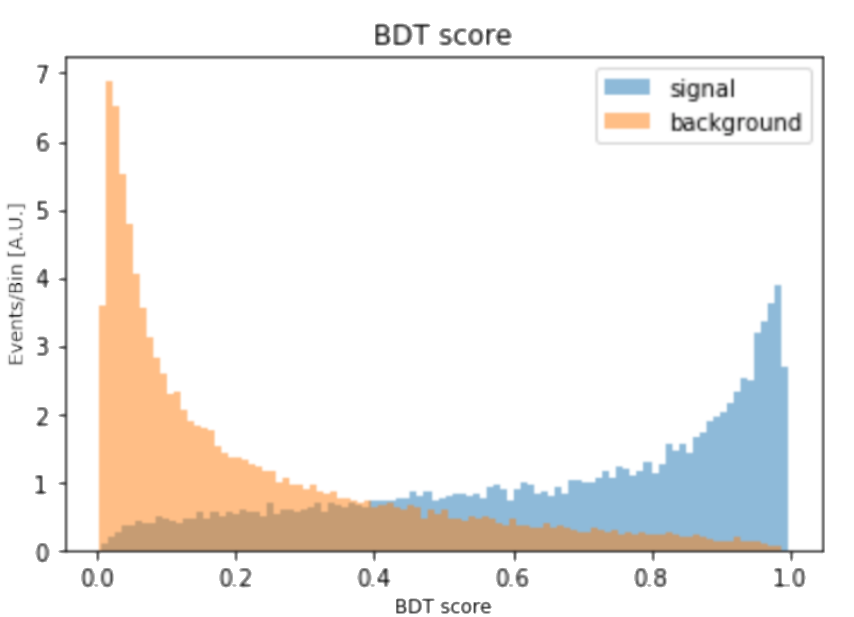
\includegraphics[width=3in]{BDT/bdt_pred_v2}
\caption{Signal predictions of the trained BDT for independent signal and background samples not used for training.}
\label{fig:bdt_pred}
\end{center}
\end{figure}

The predictions from the optimized BDT are shown in Figure~\ref{fig:bdt_pred}. A maximum significance of 1.84$\pm$0.09 was obtained, yielding $986.3 \pm 8.9$ signal events and 2.8$\pm 0.1$ $\cdot$ $10^5$ background events. 
